%% Packages initialisation
\documentclass[10pt,compress]{beamer}
\usepackage[utf8]{inputenc}               % Enable UTF-8 compatible typing
\usepackage{hyperref}                     % Interactive PDF
\usepackage{tikz}
\usetikzlibrary{fit,calc,trees,positioning,arrows,chains,shapes.geometric,%
    decorations.pathreplacing,decorations.pathmorphing,shapes,%
    matrix,shapes.symbols,intersections}


%% Use the default theme
\usetheme{Madrid}

%% Colours block environment headings
% \useinnertheme{rectangles}
% \mode<beamer>{\setbeamertemplate{blocks}[rounded][shadow=false]} 
% \setbeamercolor{block title}{bg=blue!10,fg=black}
% \makeatletter
% \pgfdeclareverticalshading[lower.bg,upper.bg]{bmb@transition}{200cm}{%
%   color(0pt)=(upper.bg); color(2pt)=(upper.bg); color(4pt)=(upper.bg)}
% \makeatother

%% Enable slide numbering
\makeatletter
\setbeamertemplate{footline}
{
  \leavevmode%
  \hbox{%
  \begin{beamercolorbox}[wd=.3\paperwidth,ht=2.25ex,dp=1ex,left]{author in head/foot}%
    \hspace*{2ex}\usebeamerfont{author in head/foot}\insertshortauthor~~\beamer@ifempty{\insertshortinstitute}{}{(\insertshortinstitute)}
  \end{beamercolorbox}%
  \begin{beamercolorbox}[wd=.5\paperwidth,ht=2.25ex,dp=1ex,center]{title in head/foot}%
    \usebeamerfont{title in head/foot}\insertshorttitle
  \end{beamercolorbox}%
  \begin{beamercolorbox}[wd=.2\paperwidth,ht=2.25ex,dp=1ex,right]{date in head/foot}%
    \usebeamerfont{date in head/foot} \usebeamerfont{date in head/foot}\insertshortdate{}\hfill \insertframenumber /\inserttotalframenumber\hspace*{2ex}
  \end{beamercolorbox}}%
  \vskip0pt%
}
\makeatother

%% Hide navigation buttons
\beamertemplatenavigationsymbolsempty

%% Listings
\usepackage{xcolor}
\usepackage{listings}

\lstset{
 backgroundcolor=\color{white},   % choose the background color; you must add \usepackage{color} or \usepackage{xcolor}
 basicstyle=\ttfamily\small,        % the size of the fonts that are used for the code
 commentstyle=\itshape,
 breakatwhitespace=false,         % sets if automatic breaks should only happen at whitespace
 breaklines=true,                 % sets automatic line breaking
 captionpos=b,                    % sets the caption-position to bottom
 deletekeywords={...},            % if you want to delete keywords from the given language
 escapeinside={§*}{*§},          % if you want to add LaTeX within your code
 extendedchars=true,              % lets you use non-ASCII characters; for 8-bits encodings only, does not work with UTF-8
 frame=none,	                   % adds a frame around the code
 keepspaces=true,                 % keeps spaces in text, useful for keeping indentation of code (possibly needs columns=flexible)
 numbers=none,                    % where to put the line-numbers; possible values are (none, left, right)
 rulecolor=\color{black},         % if not set, the frame-color may be changed on line-breaks within not-black text (e.g. comments (green here))
 showspaces=false,                % show spaces everywhere adding particular underscores; it overrides 'showstringspaces'
 showstringspaces=false,          % underline spaces within strings only
 showtabs=false,                  % show tabs within strings adding particular underscores
 tabsize=2,	                   % sets default tabsize to 2 spaces
 title=\lstname,                   % show the filename of files included with \lstinputlisting; also try caption instead of title
  belowcaptionskip=-1\baselineskip,
  xleftmargin=\parindent
}

\definecolor{darkgreen}{rgb}{0.000000,0.392157,0.000000}
\definecolor{violetred}{rgb}{0.915686,0.125490,0.364706}

% Define Links as a lst-language
\lstdefinelanguage{Links}{% 
  morekeywords={spawn, receive, typename, fun, op, var, if, this, true, false, else, case, switch, handle, handler, shallowhandler, do, sig, spawnAngel, spawnDemon, spawn},%
  sensitive=t, % 
  keywordstyle=\color{red},
  emph={Comp,Player,Bool,Int,GTree,Cheat,Zero,Choose,Rand,Move,Winner,Take,Return,Get,Put,GameState,Alice,Bob,Fail,Nothing,Just,Maybe,Toss,Heads,Tails,Process,Buyer,Coffee,Pay,Cost,Candidate,Stop,PassingComet,CelebritySighting,Float,String,Pid,EProcess,Row,Spawn,Yield,Recv,Send,FreshName,Queue,Dictionary,Myself,Type},
  emphstyle={\color{blue}},
  comment=[l]{\#},% 
  commentstyle={\itshape\color{darkgreen}},%
  escapeinside={(*}{*)},%
  morestring=[d]{"},%
  stringstyle={\color{violetred}}%
 }

% Haskell style
\lstdefinestyle{haskell}{
  language=Haskell,
  basicstyle=\linespread{1.0}\ttfamily\footnotesize,
  literate= {+}{{$+$}}1 {*}{{$*$}}1
            {<=}{{$\leq$}}1 {/=}{{$\neq$}}1 
            {==}{{$\equiv$}}1 {=>}{{$\Rightarrow$}}1
            {->}{{$\to$}}1 {<-}{{$\leftarrow$}}1
            {.}{{$\circ$}}1 {$$}{{\$}}1
}
% Ocaml style
\lstdefinestyle{ocaml}{
  language=Caml,%
  morekeywords={effect, perform},%
  emph={Obj,Choose},%
%  literate= {+}{{$+$}}1 {*}{{$*$}}1
%            {<=}{{$\leq$}}1 {>=}{{$\geq$}}1 {<>}{{$\neq$}}1 
%            {==}{{$\equiv$}}1 {=>}{{$\Rightarrow$}}1
%            {->}{{$\to$}}1
}

\usepackage{textcomp}
%\newcommand{\textapprox}{{\fontfamily{ptm}\selectfont\texttildelow}}
%\newcommand{\wildarrow}{\linksify{\textapprox{}>}}
\newcommand{\wildarrow}{\fontfamily{ptm}\selectfont\linksify{\textasciitilde{}>}}
% Links style
\lstdefinestyle{links}{
  caption={},
  basicstyle=\linespread{1.0}\ttfamily\footnotesize,
  language=Links,
  literate= {~>}{{\wildarrow}}1
}

\lstset{style={links}}

% Terminal / prompt style
\lstdefinestyle{terminal}{
  caption={},
  basicstyle=\linespread{1.0}\ttfamily\footnotesize,
  keywordstyle={},
  emphstyle={},
  commentstyle={}
}

%% Meta information
\author[D. Hillerström]{Daniel Hillerström \inst{1} \and Sam Lindley \inst{1} \and KC Sivaramakrishnan \inst{2}}
\title{Compiling Links Effect Handlers to the OCaml Backend}
\institute[University of Edinburgh]{\inst{1} The University of Edinburgh, UK \and \inst{2} University of Cambridge, UK}
\subtitle{ML Workshop '16}
\date[22-09-2016]{September 22, 2016}

%% Slides
\begin{document}
% Sponsors slide
\begin{frame}[plain]
\frametitle{This work is supported by}
\begin{columns}[T]
\begin{column}{0.5\textwidth}
\begin{figure}

\includegraphics[scale=0.6]{figures/uoe.eps}
\end{figure}
\end{column}
\hfill
\begin{column}{0.5\textwidth}
\begin{figure}

\includegraphics[scale=0.6]{figures/school_of_informatics.eps}
\end{figure}
\end{column}
\end{columns}

\vfill

\begin{columns}[T]
\begin{column}{0.5\textwidth}
\begin{figure}

\includegraphics[scale=0.35]{figures/cdtppar.eps}
\end{figure}
\end{column}
\hfill
\begin{column}{0.5\textwidth}
\begin{figure}

\includegraphics[scale=0.3]{figures/epsrc.eps}
\end{figure}
\end{column}
\end{columns}

\vfill

\begin{columns}[T]
\begin{column}{0.5\textwidth}
\begin{figure}

\includegraphics[scale=0.18]{figures/cambridge.eps}
\end{figure}
\end{column}
\hfill
\begin{column}{0.5\textwidth}
\begin{figure}
OCaml Labs
\end{figure}
\end{column}
\end{columns}

\end{frame}

% Title slide
\begin{frame}[plain]
  \maketitle
\end{frame}

%% Introduction of Links
\begin{frame}
\frametitle{The Programming Language Links}
Meet Links (Cooper et al., 2006)
\begin{itemize}
  \item a ML-like strict functional programming language,
  \item a single-source language for multi-tier web-programming,
  \item with a syntax reminiscent of JavaScript, e.g. \lstinline$fun foo(x,y) \{ ... \}$,
  \item and a strong type system including linear types,
  \item with effect typing based on row polymorphism,
  \item and it provides \emph{effect handlers} for controlling effects (Hillerström, 2015).
\end{itemize}
Links has three backends, each written in OCaml:
\begin{itemize}
 \item a JavaScript compiler for the client,
 \item an interpreter for the server,
 \item and an SQL generator for the database,
 \item and with this work a compiler for the server.
\end{itemize}
See more at \url{http://www.links-lang.org}.
\end{frame}

%% Introduction of handlers
\begin{frame}[fragile]
\frametitle{Algebraic Effects and Abstract Computations}
An algebraic effect is a collection of \emph{abstract operations}, e.g.

\[ 
Nondet = \{\text{\lstinline$Choose : Bool$}\}, \qquad Failure = \{\text{\lstinline$Fail : Zero$}\}
\]

Using these operations we can define effectful computations \emph{abstractly}, e.g.
\begin{onlyenv}<1-1>
\begin{lstlisting}

fun toss() { if (do Choose) Heads else Tails }
\end{lstlisting}
\end{onlyenv}
%
% \begin{onlyenv}<2-2>
% \begin{lstlisting}

% fun toss() { if (choose()) Heads else Tails }
% \end{lstlisting}
% \end{onlyenv}
%
\begin{onlyenv}<2-3>
\begin{lstlisting}
sig toss : () {Choose:Bool|e}-> Toss
fun toss() { if (do Choose) Heads else Tails }
\end{lstlisting}
\end{onlyenv}
%

% Algebraic effects compose seamlessly, e.g.
% \begin{onlyenv}<1-1>
% \begin{lstlisting}

% fun drunkToss() { if (do Choose) toss() else switch (do Fail) { } }
% \end{lstlisting}
% \end{onlyenv}
%
% \begin{onlyenv}<2-2>
% \begin{lstlisting}

% fun drunkToss() { if (choose()) toss() else fail() }
% \end{lstlisting}
% \end{onlyenv}
% %
% \begin{onlyenv}<3-4>
% \begin{lstlisting}
% sig drunkToss : () {Choose:Bool,Fail:Zero|e}-> Toss
% fun drunkToss() { if (choose()) toss() else fail() }
% \end{lstlisting}
% \end{onlyenv}

\begin{uncoverenv}<3-3>
Evaluation of an abstract computation\dots
\begin{lstlisting}[style=terminal]
links> toss();
*** Error: Unhandled operation: Choose
\end{lstlisting}
\dots but, what is the semantics of \lstinline$Choose$?
\end{uncoverenv}

\end{frame}

\begin{frame}[fragile]
  \frametitle{Abstract Operation Instantiation with Handlers} 
%
  A handler instantiates abstract operations with concrete
  implementations, e.g.
%% Random result animation
\begin{onlyenv}<1-1>
\begin{lstlisting}


handler randomResult {
  case Return(x) -> x
  case Choose(resume) -> resume(random() > 0.5)
}
\end{lstlisting}
\end{onlyenv}
%
\begin{onlyenv}<2-3>
\begin{lstlisting}
sig randomResult : (() {Choose:Bool|e}-> a) -> 
                    () {Choose{p}  |e}-> a
handler randomResult {
  case Return(x) -> x
  case Choose(resume) -> resume(random() > 0.5)
}
\end{lstlisting}
\end{onlyenv}
%
%% All results animation
\begin{onlyenv}<4->
\begin{lstlisting}
sig allChoices : (() {Choose:Bool|e}->  a) -> 
                  () {Choose{p}  |e}-> [a]
handler allChoices {
  case Return(x) -> [x]
  case Choose(resume) -> resume(true) ++ resume(false)
}
\end{lstlisting}
\end{onlyenv}
%
The function \lstinline$resume$ is the captured (delimited) continuation of the operation.
\vfill
\begin{onlyenv}<3->
Interpretation of \lstinline$toss$ with this handler:
\begin{onlyenv}<3-3>
\begin{lstlisting}[style=terminal]
links> randomResult(toss)();
Tails : Toss
\end{lstlisting}
\end{onlyenv}
%
\begin{onlyenv}<4->
\begin{lstlisting}[style=terminal]
links> allChoices(toss)();
[Heads, Tails] : [Toss]
\end{lstlisting}
\end{onlyenv}
\end{onlyenv}

% \begin{onlyenv}<5-5>
% Interpretation of \lstinline$drunkToss$ with either handler:
% \begin{lstlisting}[style=terminal]
% links> allChoices(drunkToss)();
% *** Error: Unhandled operation: Fail
% \end{lstlisting}
% \end{onlyenv}
\end{frame}

\begin{frame}[fragile]
  \frametitle{Handlers can be Abstract Too}
  Consider the following abstract handler:
\begin{lstlisting}
sig flip : (() {Choose:Bool |e}-> a) ->
            () {Choose:Bool |e}-> a)
handler flip {
  case Return(x)      -> x
  case Choose(resume) -> resume(not(do Choose))
}
\end{lstlisting}
We may use \lstinline$allChoices$ to interpret \lstinline$flip(toss)$:
\begin{lstlisting}[style=terminal]
links> allChoices(flip(toss))();
[Tails, Heads] : [Toss]  
\end{lstlisting}
\end{frame}


% \begin{frame}[fragile]
% \frametitle{Exception Handling}
% %
% We can define a handler for \lstinline$Fail$ independently, e.g.
% %
% \begin{lstlisting}
% sig maybeResult : (() {Fail:Zero|e}->       a) ->
%                    () {Fail{_}  |e}-> Maybe(a)
% handler maybeResult {
%   case Return(x) -> Just(x)
%   case Fail(_)   -> Nothing
% }
% \end{lstlisting}
% %
% Impossible to invoke the continuation because \lstinline$Fail$ expects
% a value of \lstinline$Zero$. Thus, this handler amounts to an \emph{exception handler}.
% \vfill
% Handlers compose to fully interpret an abstract computation, e.g.
% \begin{onlyenv}<1-1>
% \begin{lstlisting}[style=terminal]
% links> maybeResult(allChoices(drunkToss))();
% Nothing : Maybe([Toss])
% \end{lstlisting}
% \end{onlyenv}
% %
% \begin{onlyenv}<2-2>
% \begin{lstlisting}[style=terminal]
% links> allChoices(maybeResult(drunkToss))();
% [Just(Heads), Just(Tails), Nothing] : [Maybe(Toss)]
% \end{lstlisting}
% \end{onlyenv}
% \end{frame}

% \begin{frame}[fragile]
%   \frametitle{Classification of Handlers}
% Exception handlers
% \hrule
% \begin{columns}
% \begin{column}{0.6\textwidth}
% \begin{lstlisting}
% handler maybeResult {
%   case Return(x) -> Just(x)
%   case Fail(_)   -> Nothing
% }
% \end{lstlisting}
% \end{column}
% \hfill
% \begin{column}{0.4\textwidth}
% Zero invocations of the continuation.
% \end{column}
% \end{columns}
% %

% Linear handlers
% \hrule
% \begin{columns}
% \begin{column}{0.6\textwidth}
% \begin{lstlisting}
% handler randomResult {
%   case Return(x)      -> x
%   case Choose(resume) -> 
%      resume(random() > 0.5)
% }
% \end{lstlisting}
% \end{column}
% \hfill
% \begin{column}{0.4\textwidth}
% Linear consumption of the continuation.
% \end{column}
% \end{columns}

% Multi-shot handlers
% \hrule
% \begin{columns}
% \begin{column}{0.6\textwidth}
% \begin{lstlisting}
% handler allChoices {
%   case Return(x)      -> [x]
%   case Choose(resume) -> 
%      resume(true) ++ resume(false)
% }
% \end{lstlisting}
% \end{column}
% \hfill
% \begin{column}{0.4\textwidth}
% Multiple consumptions of the continuation.
% \end{column}
% \end{columns}
% Exception and linear handlers are also known as \emph{affine} handlers.
% \end{frame}

\begin{frame}
  \frametitle{Classification of Handlers}
Handlers can be classified according to their continuation consumption.
  \begin{table}
    \begin{tabular}{| l | r |}
      \hline
      Type & Cont. consumption \\
      \hline
      Exception handler & $0$ \\
      \hline
      Linear handler    & $1$ \\
      \hline
      Multi-shot handler & $> 1$ \\
      \hline
    \end{tabular}
  \end{table}
\end{frame}

%% Compiling handlers
\begin{frame}
  \frametitle{Aim}

  Handlers are not only for coin tossing. In
  particular, we have a reconstruction of the concurrency model of
  Links using handlers (Hillerström, 2016).
  
  \vspace{1cm}
  
  Thus we are interested in making this abstraction efficient and safe
  while retaining modularity.
\end{frame}

% \begin{frame}
%   \frametitle{Compiling Handlers}
% Compilation options
% \begin{itemize}
%   \item Continuation monad (Kammar et al., 2013)
%   \item Free monad (Bauer and Pretnar, 2015)
%   \item \alt<2>{\tikz[baseline,remember picture]{\node[fill=green!20,anchor=base,rounded corners=2pt] (t1){Direct-style like Multicore OCaml (Dolan et al., 2015).};}}{Direct-style like Multicore OCaml (Dolan et al., 2015).}
% %  \item Full CPS translation
%   \item Selective CPS translation (Leijen, 2016)
% \end{itemize}
% \end{frame}

%% Compiler backend overview
\begin{frame}[fragile]
  \frametitle{Compiler Backend}
\begin{figure}
\tikzset{my rectangle/.style={
        draw=black,
        thick, 
        rectangle, 
        minimum width={width("OCaml frontend")+2pt}}
}
\centering
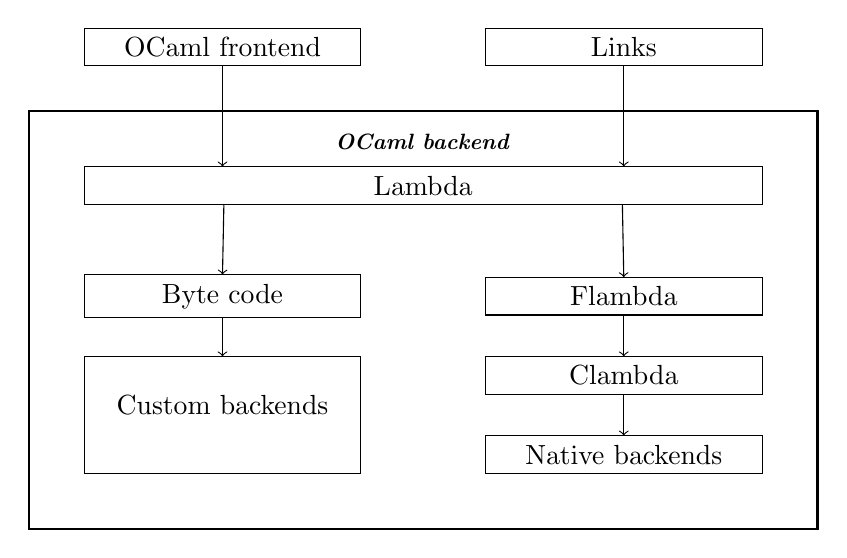
\begin{tikzpicture}[node distance=5pt,every node/.style={draw, minimum width=100pt, outer sep=0pt}]

  \node(A)          {OCaml frontend};
  \node(B)[right=of A,xshift=40pt] {Links};

  \node(C)[inner sep=0pt,yshift=-50pt,fit={(A) (B)},label=center:Lambda] {};

  \node[above=of C,draw=none,yshift=-2pt] {\footnotesize{\textbf{\textit{OCaml backend}}}};

  \node(D)[yshift=-90pt]          {Byte code};
  \node(E)[right=of D,xshift=40pt] {Flambda};

  \node(G)[below=of E,yshift=-10pt] {Clambda};
  \node(H)[below=of G,yshift=-10pt] {Native backends};

  \node(F)[fit=(G)(H),inner sep=0,left=of G.north west,anchor=north east,xshift=-40pt]          {Custom backends};


  \node(Z)[thick,fit=(C)(H),inner sep=20pt] {};

  \draw[->] (A.south) to ([xshift=50pt]C.north west);
  \draw[->] (B.south) to ([xshift=-50pt]C.north east);

  \draw[->] ([xshift=-72pt]C.south) to (D.north);

  \draw[->] (D) to (F);

  \draw[->] ([xshift=72pt]C.south) to (E.north);
  \draw[->] (E) to (G);
  \draw[->] (G) to (H);
%  \node(C)[below=of B] {C};
%  \node(D)[below=of C] {D};

%  \node(Z)[fit=(A)(D),right=of A.north east,anchor=north west, inner sep=0] {Z};

% % Frontends
% \node [my rectangle] (OCaml frontend) at (0,0) {OCaml frontend};
% \node [my rectangle] (Links frontend) at (6,0) {Links frontend};

% % OCaml backend
% \node [my rectangle,minimum width=270pt] (Lambda) at (3,-2) {Lambda};
% %\node[rectangle,draw=black,ultra thick,minimum height=+5.0cm,minimum width=+4.0cm,fit ={(Parser.north) (Typechecker.south)}] (Frontend) {};
\end{tikzpicture}
\end{figure}
\end{frame}

\begin{frame}[fragile]
  \frametitle{Multicore OCaml Handlers}
%
Multicore OCaml
\begin{itemize}
\item provides effect handlers as abstraction for concurrency,
\item provides an efficient, native implementation of \emph{linear} effect handlers,
\item provides an explicit copying construct for on demand multi-shot handlers.
%\item and implements handlers as heap-managed stack data structures.
\end{itemize}

Consider the following example in Links and OCaml:
\begin{lstlisting}[style=terminal]
links> allChoices(flip(toss))()
[Tails, Heads] : [Toss]  
\end{lstlisting}      

\begin{onlyenv}<1-1>    
\begin{lstlisting}[style=terminal]
ocaml# allChoices (flip toss) ();;

\end{lstlisting}
\end{onlyenv}
%
\begin{onlyenv}<2->    
\begin{lstlisting}[style=terminal]
ocaml# allChoices (flip toss) ();;
Exception: Invalid_argument "continuation already taken".
\end{lstlisting}
\end{onlyenv}

% Runtime layout of \lstinline$randomResult(maybeResult(drunkToss))$:
% \begin{figure}
% \tikzset{stack/.style={
%         draw=black, 
%         rectangle, 
%         minimum width=18pt,
%         minimum height=55pt,
%         fill=blue!75}
% }

% \tikzset{handler/.style={
%         draw=black, 
%         rectangle, 
%         minimum width=18pt,
%         minimum height=15pt,
%         fill=green!75}
% }
% \begin{tikzpicture}[node distance=0pt,every node/.style={draw, rectangle,  minimum width=10pt, outer sep=0pt}]

% \node [stack] (s1) { };
% \node [handler,above=of s1] (h1) { $H_1$ };
% \node [draw=none,below=of s1,yshift=-20pt] (oplabel) { Handles \lstinline$Choose$ };

% \node [draw=none,left=of h1,xshift=-20pt,yshift=-10pt] (h1label) {handler};

% \node [stack,right=of s1,xshift=70pt] (s2) { };
% \node [handler,above=of s2] (h2) { $H_2$ };

% \node [stack,right=of s2,xshift=70pt] (s3) { };

% \node [draw=none,below=of s3,yshift=-20pt] (drunkToss) { \lstinline$drunkToss$ computation };

% \node [draw=none,above=of s3,yshift=25pt] (ghost1) { };
% \node [draw=none,right=of ghost1,xshift=15pt] (ghost2) { call chain };
% \node [draw=none,above=of ghost1,yshift=5pt] (ghost3) { };
% \node [draw=none,right=of ghost3,xshift=15pt] (ghost4) { reference };
% \draw[dotted,thick,->] (ghost1) -- (ghost2) { };
% \draw[thick,->] (ghost3) -- (ghost4) { };

% \uncover<2-2>{\node [draw=none,left=of s3,yshift=30pt,xshift=-5pt] {\lstinline$do Choose$};}
% \uncover<5-5>{\node [draw=none,left=of s3,yshift=30pt,xshift=5pt] {\lstinline$resume(true)$};}
% \uncover<2-5>{\draw[thick,->] (h2) -- (s3) { };}

% \uncover<3-3>{\node [draw=none,left=of h2,xshift=-2pt,yshift=6pt] {forward \lstinline$Choose$};}
% \uncover<4-4>{\node [draw=none,left=of h2,xshift=-2pt,yshift=6pt] {\lstinline$resume(true)$};}
% \uncover<3-4>{\draw[thick,->] (h1) -- (h2) { };}

% % Arrows
% \draw[->,thick] ([yshift=-10pt]s2.west) -- ([yshift=-10pt]s1.east) { };
% \draw[dotted,thick,->] (h1.east) [in=180,out=0] to ([yshift=2pt]s2.south west) { };
% \draw[->] (h1label.east) -- (h1.west) { };

% \draw[->,thick] ([yshift=-10pt]s3.west) -- ([yshift=-10pt]s2.east) { };
% \draw[dotted,thick,->] (h2.east) [in=180,out=0] to ([yshift=2pt]s3.south west) { };

% \draw[->,draw=red!90,thick] (oplabel) [in=-95,out=80] to (h1) { };
% \draw[->,draw=red!90,thick] (drunkToss) [in=-95,out=80] to (s3.south) { };
% \end{tikzpicture}
% \end{figure}
\end{frame}

\begin{frame}
  \frametitle{On Demand Multi-shot Handlers are a Fragile Abstraction}
Runtime layout of \lstinline$allChoices(flip(toss))$:
\begin{figure}
\tikzset{stack/.style={
        draw=black, 
        rectangle, 
        minimum width=18pt,
        minimum height=55pt,
        fill=blue!75}
}

\tikzset{handler/.style={
        draw=black, 
        rectangle, 
        minimum width=18pt,
        minimum height=15pt,
        fill=green!75}
}
\begin{tikzpicture}[node distance=0pt,every node/.style={draw, rectangle,  minimum width=10pt, outer sep=0pt}]

\node [stack] (s1) { };
\node [handler,above=of s1] (h1) { $H_1$ };
\node [draw=none,below=of s1,yshift=-20pt] (allChoices) { \lstinline$allChoices$ };

\node [draw=none,left=of h1,xshift=-20pt,yshift=-10pt] (h1label) {handler};

\node [stack,right=of s1,xshift=70pt] (s2) { };
\node [handler,above=of s2] (h2) { $H_2$ };
\node [draw=none,below=of s2,yshift=-20pt] (flip) { \lstinline$flip$ };

\node [stack,right=of s2,xshift=70pt] (s3) { };

\node [draw=none,below=of s3,yshift=-20pt] (drunkToss) { \lstinline$toss$ computation };

\node [draw=none,above=of s3,yshift=25pt] (ghost1) { };
\node [draw=none,right=of ghost1,xshift=15pt] (ghost2) { call chain };
\node [draw=none,above=of ghost1,yshift=5pt] (ghost3) { };
\node [draw=none,right=of ghost3,xshift=15pt] (ghost4) { reference };
\draw[dotted,thick,->] (ghost1) -- (ghost2) { };
\draw[thick,->] (ghost3) -- (ghost4) { };

\uncover<2-2>{\node [draw=none,left=of s3,yshift=30pt,xshift=-5pt] {\lstinline$do Choose$};}
\uncover<5-5>{\node [draw=none,left=of s3,yshift=30pt,xshift=5pt] {\lstinline$resume(false)$};}
\uncover<2-5>{\draw[thick,->] (h2) -- (s3) { };}

\uncover<3-3>{\node [draw=none,left=of h2,xshift=-10pt,yshift=6pt] {\lstinline$do Choose$};}
\uncover<4-4>{\node [draw=none,left=of h2,xshift=-2pt,yshift=6pt] {\lstinline$resume(true)$};}
\uncover<6-6>{\node [draw=none,left=of h2,xshift=-2pt,yshift=2pt] {\lstinline$resume(false)$};}
\uncover<3-4>{\draw[thick,->] (h1) -- (h2) { };}
\uncover<3-6>{\draw[thick,->,] ([yshift=-4pt]h1.east) to ([yshift=-4pt]h2.west) { };}

% Arrows
\draw[->,thick] ([yshift=-10pt]s2.west) -- ([yshift=-10pt]s1.east) { };
\draw[dotted,thick,->] (h1.east) [in=180,out=0] to ([yshift=2pt]s2.south west) { };
\draw[->] (h1label.east) -- (h1.west) { };

\draw[->,thick] ([yshift=-10pt]s3.west) -- ([yshift=-10pt]s2.east) { };
\draw[dotted,thick,->] (h2.east) [in=180,out=0] to ([yshift=2pt]s3.south west) { };

\draw[->,draw=red!90,thick] (allChoices) [in=-95,out=80] to (h1) { };
\draw[->,draw=red!90,thick] (flip) [in=-95,out=80] to (h2) { };
\draw[->,draw=red!90,thick] (drunkToss) [in=-95,out=80] to (s3.south) { };

% Stack pointers
\uncover<1-1,5-5>{\node [draw=none,right=of s3,xshift=15pt,yshift=35pt] (sp1) { sp };}
\uncover<1-1,5-5>{\draw[->,thick] (sp1.west) to (s3.north east) { };}

\uncover<2-2,4-4,7-7>{\node [draw=none,right=of h2,xshift=15pt,yshift=15pt] (sp2) { sp };}
\uncover<2-2,4-4,7-7>{\draw[->,thick] (sp2.west) to (h2.north east) { };}

\uncover<3-3,6-6>{\node [draw=none,right=of h1,xshift=15pt,yshift=15pt] (sp3) { sp };}
\uncover<3-3,6-6>{\draw[->,thick] (sp3.west) to (h1.north east) { };}

\uncover<8->{\node[starburst, draw, minimum width=7cm, minimum height=5cm,red,fill=orange,line width=1.5pt,above=of flip]
{\Huge{BOOM!}};}

\end{tikzpicture}
\uncover<9->{\textbf{Conservative solution:} Implement every handler as a multi-shot handler.}
\end{figure}
\end{frame}

% \begin{frame}
%   \frametitle{Translating Links Handlers to OCaml Handlers (1)}
%   \begin{table}
%     \bgroup
%     \def\arraystretch{2.5}
%    \begin{tabular}{l p{3cm} l}
%      \textbf{Links} & \hfill & \textbf{OCaml} \\
%      \hline
%      Exception handlers & \tikz[remember picture] \node[coordinate] (n1) {}; \hfill \tikz[remember picture] \node[coordinate] (n2) {}; & Exception handlers \\
%      Linear handlers    & \tikz[remember picture] \node[coordinate] (m1) {}; \hfill \tikz[remember picture] \node[coordinate] (m2) {}; & Linear handlers \\
%      Multi-shot handlers & \tikz[remember picture] \node[coordinate] (p1) {}; \hfill \tikz[remember picture] \node[coordinate] (p2) {}; & \alt<2->{On demand multi-shot handlers}{???}
%    \end{tabular}
%    \egroup
%   \end{table}
% %
% \begin{tikzpicture}[remember picture,overlay]   %% use here too
%    \path[draw=black,thick,->] ([yshift=3]n1.east) to [out=0, in=0,distance=0in] ([yshift=3]n2.east);
%    \path[draw=black,thick,->] ([yshift=3]m1.east) to [out=0, in=0,distance=0in] ([yshift=3]m2.east);
%    \path[draw=black,thick,->] ([yshift=3]p1.east) to [out=0, in=0,distance=0in] ([yshift=3]p2.east);
% \end{tikzpicture}
% \end{frame}

% \begin{frame}[fragile]
%   \frametitle{On Demand Multi-shot Handlers are Fragile} 
% %
%   Here is the \emph{multi-shot} handler \lstinline$allChoices$ with
%   explicit continuation copying:
% \begin{lstlisting}
% handler allChoices {
%   case Return(x)      -> [x]
%   case Choose(resume) -> 
%     fun multiResume(x) { var r = clone(resume); r(x) }     
%     multiResume(true) ++ multiResume(false)
% }    
% \end{lstlisting}
% %
% \begin{uncoverenv}<2->
% Consider another \emph{linear} handler for \lstinline$Choose$:
% \begin{lstlisting}
% handler flip {
%   case Return(x)      -> x
%   case Choose(resume) -> (*\alt<4->{\tikz[baseline,remember picture]{\node[fill=green!20,anchor=base,rounded corners=2pt] (t1){resume};}}{resume}*)(not(do Choose))
% }    
% \end{lstlisting}
% OCaml implements \lstinline$resume$ as a linear continuation. Consider
% what happens when we evaluate the composition
% \lstinline[mathescape]!allChoices(flip($\cdot$))!:
% \end{uncoverenv}
% %
% \begin{uncoverenv}<3->
% \begin{lstlisting}
% links> allChoices(flip(toss))();
% Exception: Invalid_argument "continuation(*\tikz[remember picture] \node[coordinate] (n1) {};*) already taken".}
% \end{lstlisting}
% \end{uncoverenv}
% %

% \begin{tikzpicture}[remember picture,overlay]   %% use here too
%    \path[draw=red,thick,->]<4-> ([yshift=2mm,xshift=-30]n1.north) to [out=80, in=270,distance=0.5in] (t1.south);
% \end{tikzpicture}
% %
% \end{frame}

% \begin{frame}
%   \frametitle{Translating Links Handlers to OCaml Handlers (2)}
%   In the light of the previous slide\dots
%   \begin{table}
%     \bgroup
%     \def\arraystretch{2.5}
%    \begin{tabular}{l p{3cm} l}
%      \textbf{Links} & \hfill & \textbf{OCaml} \\
%      \hline
%      Exception handlers & \tikz[remember picture] \node[coordinate] (n1) {}; \hfill \tikz[remember picture] \node[coordinate] (n2) {}; & Exception handlers \\
%      Linear handlers    & \tikz[remember picture] \node[coordinate] (m1) {}; \hfill \tikz[remember picture] \node[coordinate] (m2) {}; & Linear handlers \\
%      Multi-shot handlers & \tikz[remember picture] \node[coordinate] (p1) {}; \hfill \tikz[remember picture] \node[coordinate] (p2) {}; & On demand multi-shot handlers
%    \end{tabular}
%    \egroup
%   \end{table}
% %
% \uncover<2->{Clearly this is not good for performance\dots}
% %
% \begin{tikzpicture}[remember picture,overlay]   %% use here too
%    \path[draw=black,thick,->] ([yshift=3]n1.east) to [out=0, in=0,distance=0in] ([yshift=3]n2.east);
%    \alt<2->{\path[draw=black,thick,->] ([yshift=3]m1.east) to [out=0, in=0,distance=0in] ([yshift=3]p2.east);}{\path[draw=black,thick,->] ([yshift=3]m1.east) to [out=0, in=0,distance=0in] ([yshift=3]m2.east);}
%    \path[draw=black,thick,->] ([yshift=3]p1.east) to [out=0, in=0,distance=0in] ([yshift=3]p2.east);
% \end{tikzpicture}
% \end{frame}

\begin{frame}
  \frametitle{What is the Penalty?}
  \begin{figure}
    \centering
    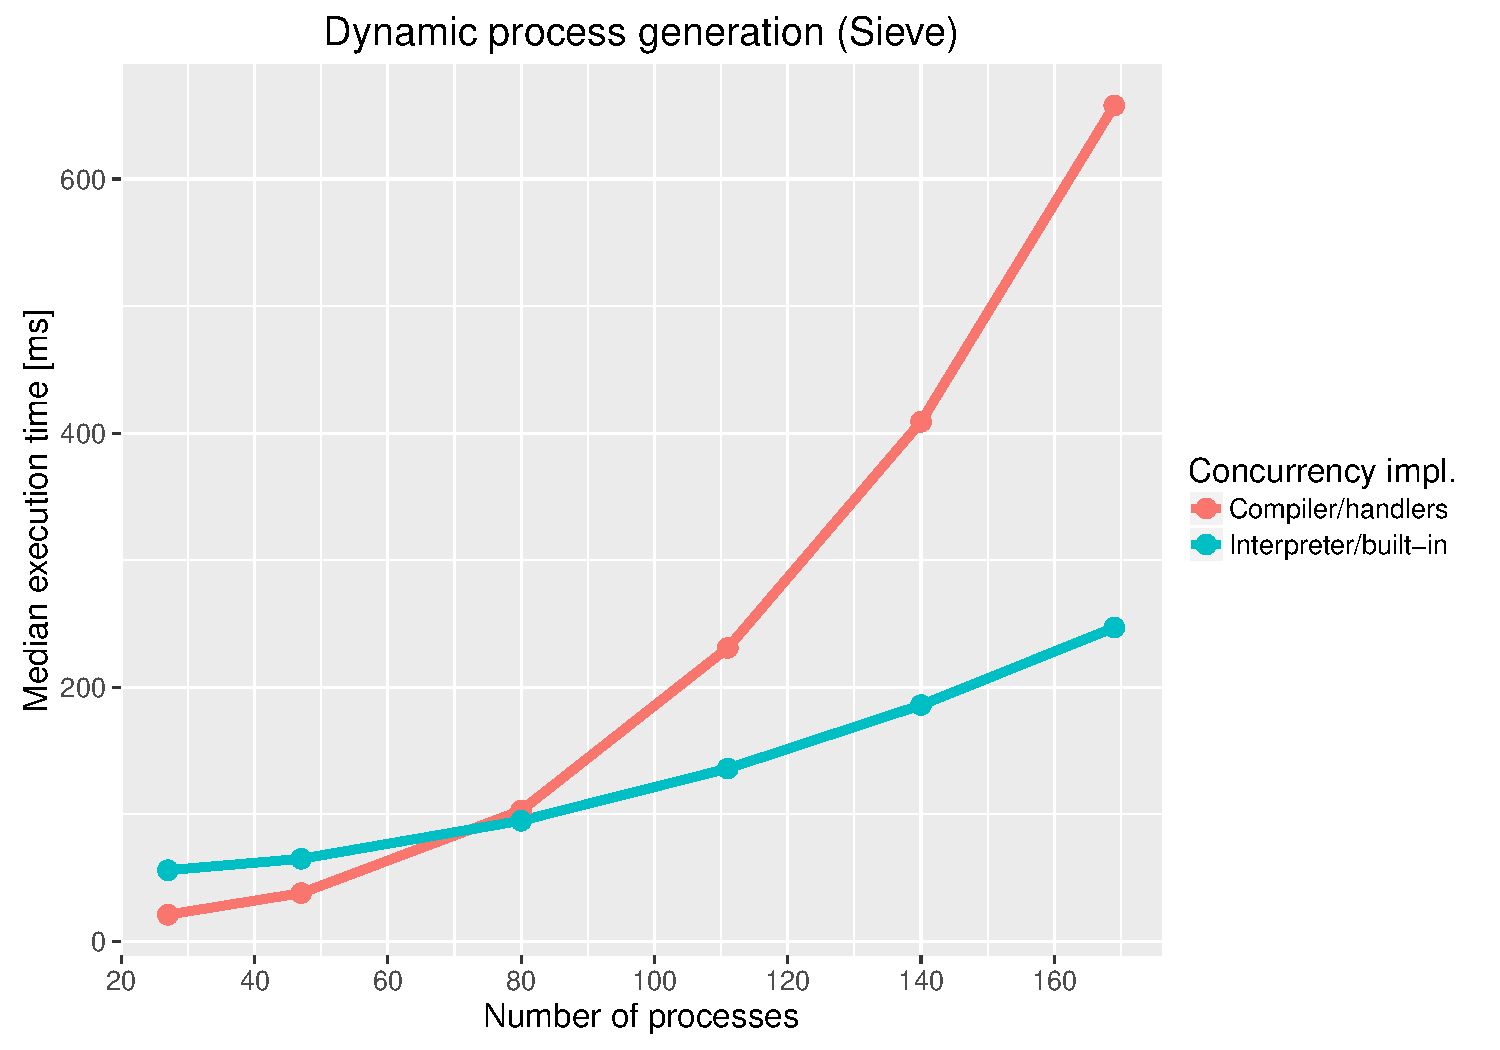
\includegraphics[scale=0.40]{figures/sieve_compiler-interpreter.pdf}
  \end{figure}
  \uncover<2->{\textbf{Idea:} Let's use the linear type system to track the linearity of handlers.}
\end{frame}

% \begin{frame}
%   \frametitle{How Can We Recover the Performance of Linear Handlers?}
%   \begin{block}{Idea}
%     Take advantage of the linear type system of Links to determine
%     whether continuations are consumed linearly. Furthermore, use the
%     effect system to track the linearity of handlers.
%   \end{block}
% Example
% \end{frame}

\begin{frame}
  \frametitle{Does It Work?}
  \begin{figure}
    \centering
    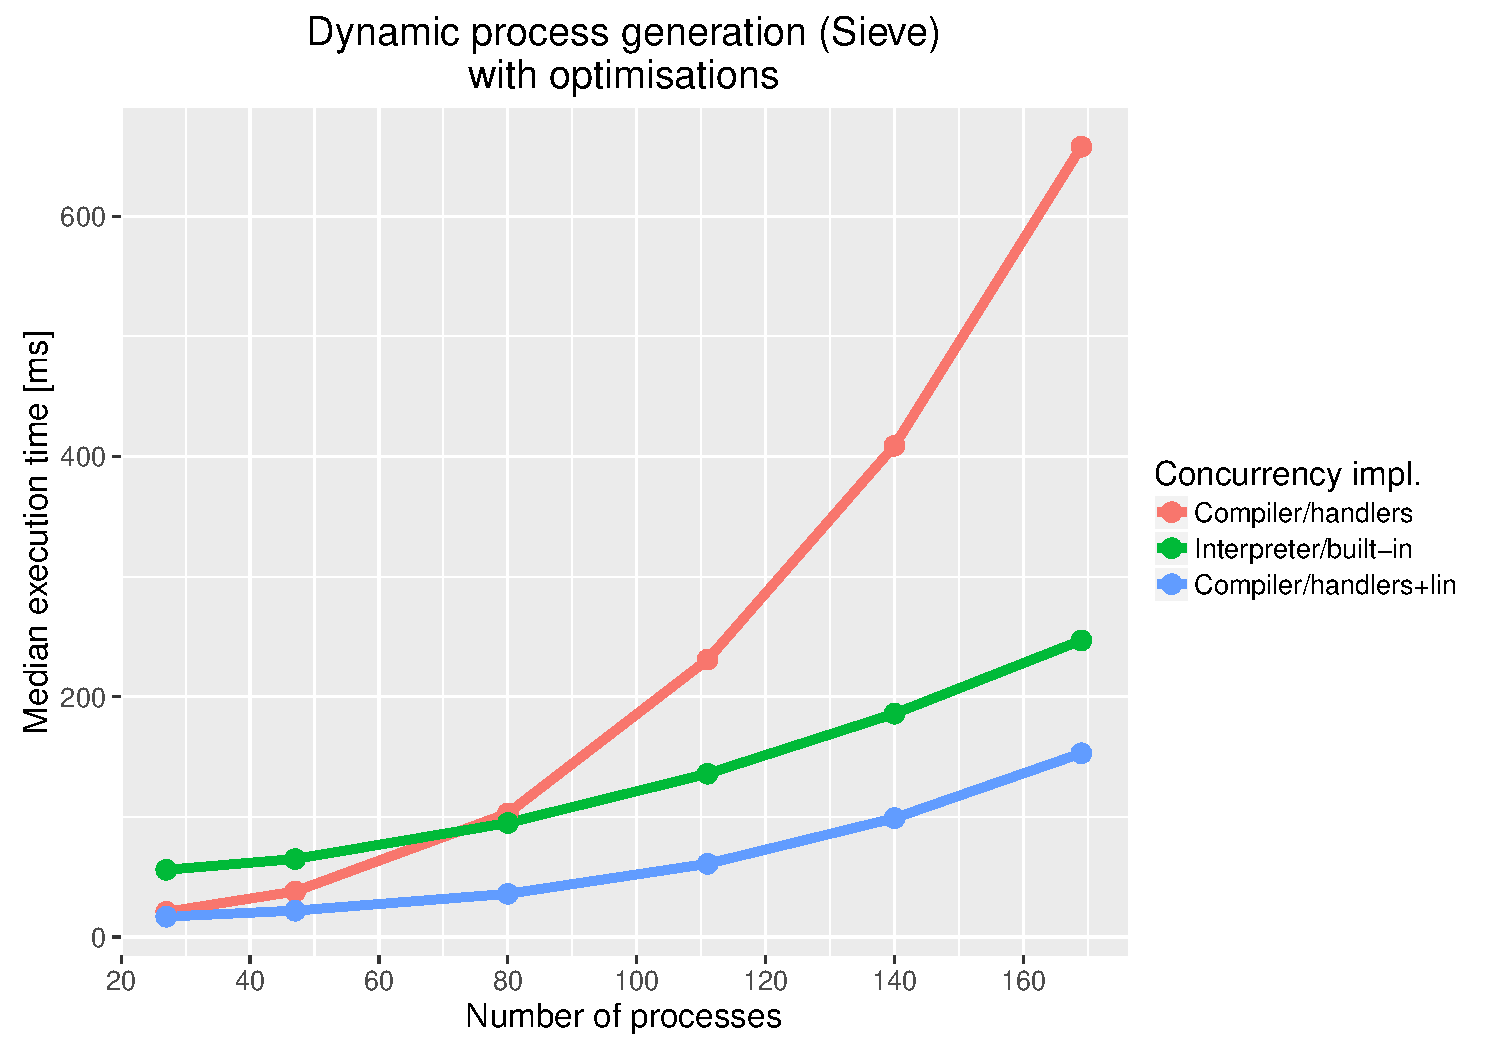
\includegraphics[scale=0.45]{figures/sieve_recovered.pdf}
  \end{figure}
\end{frame}

% \begin{frame}
%   Todo
% \begin{itemize}
%   \item Motivation for handlers
%   \item OCaml provides efficient implementation of handlers (show stack diagram)
%   \item From nice ideal world, to practical and efficient world (type-directed).
%   \item Report on optimisations
%   \item Sometime we do not want linear continuation to be promoted.
% \end{itemize}
% \end{frame}

\begin{frame}[fragile]
  \frametitle{Scoping of Handler Promotion}
  \begin{onlyenv}<1-1>
    Ideally, we want this:
  \begin{figure}
    \tikzset{handlerb/.style={
        draw=none,
        minimum width={width("h1")},
        minimum height={height("h1")}}
}
\begin{tikzpicture}
  \node (h4) [handlerb] {$h_\bot$};
  \node (h3) [handlerb,right=of h4] {$\cdots$};
  \node (h2) [handlerb,right=of h3] {$h_2^\ast$};
  \node (h1) [handlerb,right=of h2] {$h_1$};

  \node (hf1) [draw=black,rectangle,fit={(h1)}] {};
  \node (hf2) [draw=black,rectangle,fit={(hf1)(h2)}] {};
  \node (hf3) [draw=black,rectangle,fit={(hf2)(h3)}] {};
  \node (hf4) [draw=black,rectangle,fit={(hf3)(h4)}] {};
\end{tikzpicture}
\vfill
$\Rightarrow$
\vfill
\begin{tikzpicture}
  %% Transl
  \node (h4) [handlerb] {$h_\bot$};
  \node (h3) [handlerb,right=of h4] {$\cdots$};
  \node (h2) [handlerb,right=of h3] {$h_2^\ast$};
  \node (h1) [handlerb,right=of h2] {$h_1^\ast$};

  \node (hf1) [draw=black,rectangle,fit={(h1)}] {};
  \node (hf2) [draw=black,rectangle,fit={(hf1)(h2)}] {};
  \node (hf3) [draw=black,rectangle,fit={(hf2)(h3)}] {};
  \node (hf4) [draw=black,rectangle,fit={(hf3)(h4)}] {};
\end{tikzpicture}
\end{figure}
\end{onlyenv}
%
\begin{onlyenv}<2->
    But, this is what really happens:
  \begin{figure}
    \tikzset{handlerb/.style={
        draw=none,
        minimum width={width("h1")},
        minimum height={height("h1")}}
}
\begin{tikzpicture}
  \node (h4) [handlerb] {$h_\bot$};
  \node (h3) [handlerb,right=of h4] {$\cdots$};
  \node (h2) [handlerb,right=of h3] {$h_2^\ast$};
  \node (h1) [handlerb,right=of h2] {$h_1$};

  \node (hf1) [draw=black,rectangle,fit={(h1)}] {};
  \node (hf2) [draw=black,rectangle,fit={(hf1)(h2)}] {};
  \node (hf3) [draw=black,rectangle,fit={(hf2)(h3)}] {};
  \node (hf4) [draw=black,rectangle,fit={(hf3)(h4)}] {};
\end{tikzpicture}
\vfill
$\Rightarrow$
\vfill
\begin{tikzpicture}
  %% Transl
  \node (h4) [handlerb] {$h_\bot^\ast$};
  \node (h3) [handlerb,right=of h4] {$\cdots^\ast$};
  \node (h2) [handlerb,right=of h3] {$h_2^\ast$};
  \node (h1) [handlerb,right=of h2] {$h_1^\ast$};

  \node (hf1) [draw=black,rectangle,fit={(h1)}] {};
  \node (hf2) [draw=black,rectangle,fit={(hf1)(h2)}] {};
  \node (hf3) [draw=black,rectangle,fit={(hf2)(h3)}] {};
  \node (hf4) [draw=black,rectangle,fit={(hf3)(h4)}] {};
\end{tikzpicture}
\end{figure}
Need some way to capture the structure of the handler stack at the type-level.
\end{onlyenv}

\begin{table}
  \hspace{-6cm}\begin{tabular}{l l}
    \multicolumn{1}{c}{Legend} \\
    \hline
    $h_n^\ast$ & Multi-shot handler\\
    $h_n$     & Linear handler
  \end{tabular}
\end{table}
\end{frame}

\begin{frame}
  \frametitle{Channel Selection}
  The linear type system is not expressive enough to capture tombstones.
  \begin{figure}
    \begin{onlyenv}<1-2>
  \begin{tikzpicture}
    \node (ch1) [rectangle,draw=black,minimum width={width("resume")},minimum height=40pt] { resume };
    \node (ch1label) [draw=none,above=of ch1,yshift=-20pt] {$ch_1$};

    \node (choice) [draw=none,right=of ch1] { };
    
    \only<1-1>{\node (ch2) [rectangle,draw=black,minimum width={width("resume")},minimum height=40pt,right=of choice] { resume };}
    \node (ch2label) [draw=none,above=of ch2,yshift=-20pt] {$ch_2$};

    %
    \only<2->{\node (ch2) [rectangle,draw=black,minimum width={width("resume")},minimum height=40pt,right=of choice] { {\color{white}{resume}} };}
    %\only<2->{\node (ch2labelp) [draw=none,above=of ch2] {$ch_2$};}

    % Join point
    \node (pt) [circle,fill=black,draw=black,yshift=-20pt,below of=choice] { };

    \only<1-1>{\node (ghost1) [minimum width=3pt,minimum height=3pt,draw=none,below=of pt,yshift=-20pt] { $P$ };}

    \only<2-2>{\node (ghost1) [minimum width=3pt,minimum height=3pt,draw=none,below=of pt,yshift=-20pt] { $Nil$ };}
    % Arrows
    \draw[thick] (ch1.south) edge[out=300,in=180] (pt.west) { };
    \only<1-1>{\draw[thick] (ch2.south) edge[out=240,in=0] (pt.east) { };}

    \draw[thick,->] (pt.south) to (ghost1.north) { };
  \end{tikzpicture}
\end{onlyenv}
%
\begin{onlyenv}<3>
  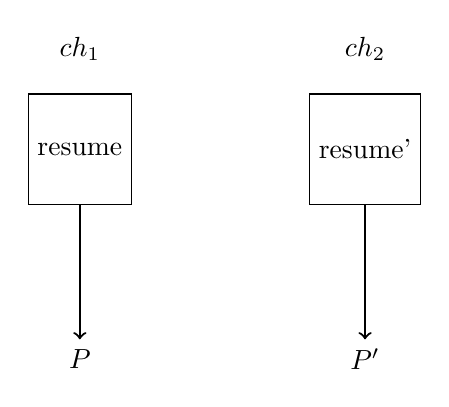
\begin{tikzpicture}
    \node (ch1) [rectangle,draw=black,minimum width={width("resume")},minimum height=40pt] { resume };
    \node (ch1label) [draw=none,above=of ch1,yshift=-20pt] {$ch_1$};

    \node (choice) [draw=none,right=of ch1] { };
    
    \node (ch2) [rectangle,draw=black,minimum width={width("resume")},minimum height=40pt,right=of choice] { resume' };
    \node (ch2label) [draw=none,above=of ch2,yshift=-20pt] {$ch_2$};

    \node (ghost1) [minimum width=3pt,minimum height=3pt,draw=none,below=of ch1,yshift=-20pt] { $P$ };

    \node (ghost2) [minimum width=3pt,minimum height=3pt,draw=none,below=of ch2,yshift=-20pt] { $P'$ };
    % Arrows
    \draw[thick,->] (ch1.south) to (ghost1.north) { };
    \draw[thick,->] (ch2.south) to (ghost2.north) { };

  \end{tikzpicture}\\
  This is not the desired semantics!
  \end{onlyenv}
\end{figure}
\end{frame}

\begin{frame}
  \frametitle{Compiling Handlers -- Related Work}
Compilation options
\begin{itemize}
  \item Continuation monad (Kammar et al., 2013)
  \item Free monad (Bauer and Pretnar, 2015)
  \item Direct-style like Multicore OCaml (Dolan et al., 2015)
  \item Selective CPS translation (Leijen, 2016)
\end{itemize}
\end{frame}

\begin{frame}
  \frametitle{Summary}
\begin{itemize}
\item Algebraic effects and handlers provide a modular abstraction for
  effectful programming.
\item Regard Links as an experimental frontend to OCaml with effect
  typing and linear types.
\item Type-directed optimisation of effect handlers\dots
\end{itemize}
\end{frame}

% Load subsequent slides, e.g.
%\input{slides/index}

% Bibliography
\bibliographystyle{unsrt}
\begin{frame}[allowframebreaks]
  \frametitle{References}
  \nocite{*}
  \bibliography{compilinghandlers}
\end{frame}
\end{document}
